\documentclass[a4paper]{article}
\usepackage[german]{babel}
\usepackage{listings}
\usepackage{appendix}
\usepackage[dvips]{graphicx}
\usepackage[dvips,a4paper=true,backref=true,hyperindex=false,colorlinks=false,pdfhighlight=/N,linkbordercolor={0 0 0}, pdfborder={0 0 0},breaklinks=true,pdftitle={Dokumentation: Wahlinformationssystem}, pdfauthor={Tobias Johann Mühlbauer, Wolf Rödiger},pdfproducer={Latex},pdfcreator={LaTex+dvips+ps2pdf}]{hyperref}
\usepackage{breakurl}\usepackage[utf8]{inputenc}
\usepackage{url}
\author{Wolf Rödiger, Tobias Mühlbauer \\ roediger at in.tum.de, muehlbau at in.tum.de}
\title{Dokumentation: Wahlinformationssystem}

\begin{document}

\maketitle

\newpage

\tableofcontents

\newpage

\section{Informationsstrukturanforderungen}

Im Folgenden sind die Objekte und Beziehungen des Wahlinformationssystems strukturell beschrieben. Angaben zur Anzahl bestimmter Objekte sind den Bestimmungen zur Bundestagswahl des Jahres 2009 entnommen.

Eine zentrale Rolle bei einer Wahl spielen die Wahlberechtigten:

\paragraph{Wahlberechtigter}
\begin{itemize}
\item Besonderheit: Exklusiv und Existenzabhängig von Wahlbezirk
\item Anzahl: 62\,168\,489
\item Attribute
	\begin{itemize}
	\item Wählerverzeichnisnummer
		\begin{itemize}
		\item Typ: integer
		\item Anzahl Wiederholungen: 0
		\item Definiertheit: 100\%
		\item Identifizierend: ja
		\end{itemize}
	\item StimmeAbgegeben
		\begin{itemize}
		\item Typ: boolean
		\item Anzahl Wiederholungen: beliebig
		\item Definiertheit: 100\%
		\item Identifizierend: nein
		\end{itemize}
	\end{itemize}
\end{itemize}

Zur geographischen Einordnung der Wahlberechtigten dient die folgende Hierachie von Objekten:

\paragraph{Bundesland}
\begin{itemize}
\item Anzahl: 16
\item Attribute
	\begin{itemize}
	\item Name
	\begin{itemize}
		\item Typ: character
		\item Länge: 50
		\item Wertebereich: Baden-Württemberg, Bayern, Berlin, Brandenburg, Bremen, Hamburg, Hessen, Mecklenburg-Vorpommern, Niedersachsen, Nordrhein-Westfalen, Rheinland-Pfalz, Saarland, Sachsen, Sachsen-Anhalt, Schleswig-Holstein, Thüringen
		\item Anzahl Wiederholungen: 0
		\item Definiertheit: 100\%
		\item Identifizierend: ja
		\end{itemize}
	\end{itemize}
\end{itemize}

\paragraph{Wahlkreis}
\begin{itemize}
\item Besonderheit: Exklusiv und Existenzabhängig von Bundesland
\item Anzahl: 299
\item Attribute
	\begin{itemize}
	\item Wahlkreisnummer
		\begin{itemize}
		\item Typ: integer
		\item Wertebereich: 1 \ldots 299
		\item Anzahl Wiederholungen: 0
		\item Definiertheit: 100\%
		\item Identifizierend: ja
		\end{itemize}
	\item Name
		\begin{itemize}
		\item Typ: character
		\item Länge: 250
		\item Anzahl Wiederholungen: beliebig
		\item Definiertheit: 100\%
		\item Identifizierend: nein
		\end{itemize}
	\end{itemize}
\end{itemize}

\paragraph{Wahlbezirk}
\begin{itemize}
\item Besonderheit: Exklusiv und Existenzabhängig von Wahlkreis
\item Anzahl: ca. 25\,000
\item Attribute
	\begin{itemize}
	\item Wahlbezirknummer
		\begin{itemize}
		\item Typ: integer
		\item Wertebereich: 1 \ldots 25\,000
		\item Anzahl Wiederholungen: 0
		\item Definiertheit: 100\%
		\item Identifizierend: ja
		\end{itemize}
	\item Name
		\begin{itemize}
		\item Typ: character
		\item Länge: 250
		\item Anzahl Wiederholungen: beliebig
		\item Definiertheit: 100\%
		\item Identifizierend: nein
		\end{itemize}
	\end{itemize}
\end{itemize}

Stimmzettel werden im System gespeichert um eine spätere Berechnung der Sitzverteilung zu gewährleisten. Da eine Zweitstimme nicht zählt, falls bei der Erststimme ein parteiloser Kandidat gewählt wurde und dieser in den Bundestag einzieht, müssen sogar Erst- und Zweitstimme mit einer Zuordnung abgebildet werden:

\paragraph{Stimmzettel}
\begin{itemize}
\item Anzahl: max. Anzahl der Wahlberechtigten
\end{itemize}

\paragraph{Erststimme}
\begin{itemize}
\item Besonderheit: Exklusiv und Existenzabhängig von Stimmzettel
\item Anzahl: max. Anzahl der Wahlberechtigten
\end{itemize}

\paragraph{Zweitstimme}
\begin{itemize}
\item Besonderheit: Exklusiv und Existenzabhängig von Stimmzettel
\item Anzahl: max. Anzahl der Wahlberechtigten
\end{itemize}

Gewählt werden können bei einer Bundestagswahl eine Landesliste einer Partei des Bundeslandes mit der Zweit- und ein Direktkandidat des Wahlkreises mit der Erststimme:

\paragraph{Partei}
\begin{itemize}
\item Anzahl: 29
\item Attribute
	\begin{itemize}
	\item Kurzbezeichnung
	\begin{itemize}
		\item Typ: character
		\item Länge: 25
		\item Wertebereich: SPD, CDU, FDP, DIE LINKE, GRÜNE, CSU, NPD, MLPD, PIRATEN, DVU, REP, ÖDP, BÜSO, DIE TIERSCHUTZPARTEI, RRP, FAMILIE, PBC, DIE VIOLETTEN, RENTNER, PSG, VOLKSABSTIMMUNG, CM, BP, DKP, ADM, FWD, ZENTRUM, FREIE UNION, DVD
		\item Definiertheit: 100\%
		\item Identifizierend: ja
	\end{itemize}
	\item Name
	\begin{itemize}
		\item Typ: character
		\item Länge: 150
		\item Wertebereich: ``Sozialdemokratische Partei Deutschlands", ``Christlich Demokratische Union Deutschlands", ``Freie Demokratische Partei", ``Die Linke", ``Bündnis 90/Die Grünen", ``Christlich-Soziale Union in Bayern", ``Nationaldemokratische Partei Deutschlands", ``Marxistisch-Leninistische Partei Deutschlands", ``Piratenpartei Deutschland", ``Deutsche Volksunion", ``Die Republikaner", ``Ökologisch-Demokratische Partei", ``Bürgerrechtsbewegung Solidarität", ``Mensch Umwelt Tierschutz", ``Rentnerinnen- und Rentner-Partei", ``Familien-Partei Deutschlands", ``Partei Bibeltreuer Christen", ``Die Violetten - Für spirituelle Politik", ``Rentner-Partei-Deutschland", ``Partei für Soziale Gleichheit, Sektion der Vierten Internationale", ``Ab jetzt…Bündnis für Deutschland, für Demokratie durch Volksabstimmung", ``Christliche Mitte – für ein Deutschland nach Gottes Geboten", ``Bayernpartei", ``Deutsche Kommunistische Partei",``Allianz der Mitte", ``Freie Wähler Deutschland", ``Deutsche Zentrumspartei – Älteste Partei Deutschlands gegründet 1870", "Freie Union", "Demokratische Volkspartei Deutschland"
		\item Definiertheit: 100\%
		\item Identifizierend: ja
	\end{itemize}
\end{itemize}
\end{itemize}

\paragraph{Kandidat}
\begin{itemize}
\item Anzahl: 
\item Attribute
	\begin{itemize}
	\item Kandidatennummer
		\begin{itemize}
		\item Typ: integer
		\item Anzahl Wiederholungen: 0
		\item Definiertheit: 100\%
		\item Identifizierend: ja
		\end{itemize}
	\item Name
		\begin{itemize}
		\item Typ: character
		\item Länge: 150
		\item Anzahl Wiederholungen: beliebig
		\item Definiertheit: 100\%
		\item Identifizierend: nein
		\end{itemize}
	\item Geburstag
		\begin{itemize}
		\item Typ: date
		\item Anzahl Wiederholungen: beliebig
		\item Definiertheit: 100\%
		\item Identifizierend: nein
		\end{itemize}
	\item Beruf
		\begin{itemize}
		\item Typ: character
		\item Länge: 200
		\item Anzahl Wiederholungen: beliebig
		\item Definiertheit: 80\%
		\item Identifizierend: nein
		\end{itemize}
	\end{itemize}
\end{itemize}

\paragraph{Landesliste}
\begin{itemize}
\item Anzahl: ca. 300
\end{itemize}

\paragraph{Listenposition}
\begin{itemize}
\item Anzahl: ca. 3000
\item Attribute
	\begin{itemize}
	\item Position
		\begin{itemize}
		\item Typ: integer
		\item Anzahl Wiederholungen: beliebig
		\item Definiertheit: 100\%
		\item Identifizierend: nein
		\end{itemize}
	\end{itemize}
\end{itemize}

Das Ergebnis der Bundestagswahl entscheidet über die Parlamentarier im Bundestag:

\paragraph{Bundestagsabgeordneter}
\begin{itemize}
\item Anzahl: 299 - 897
\end{itemize}

\section{Datenverarbeitungsanforderungen}

Es folgen exemplarisch einige Prozessbeschreibungen für das Wahlinformationssystem:

\paragraph{Eintragen von Wahlergebnissen}
\begin{itemize}
\item Häufigkeit: Nach 18 Uhr am Wahltag minütlich
\item Priorität: hoch
\item zu verarbeitende Datenmenge
\begin{itemize}
	\item mehrere Tausend Stimmzettel mit Erst- und Zweitstimmen
\end{itemize}
\end{itemize}

\paragraph{Berechnung der Sitzverteilung im Bundestag}
\begin{itemize}
\item Häufigkeit: Nach 18 Uhr am Wahltag alle 15 Minuten
\item Priorität: mittel
\item zu verarbeitende Datenmenge
\begin{itemize}
	\item alle bisher eingetragenen Zweitstimmen
\end{itemize}
\end{itemize}

\paragraph{Berechnung von Wahlkreisgewinnern}
\begin{itemize}
\item Häufigkeit: Nach 18 Uhr am Wahltag alle 15 Minuten
\item Priorität: niedrig
\item zu verarbeitende Datenmenge
\begin{itemize}
	\item alle bisher eingetragenen Erststimmen
\end{itemize}
\end{itemize}

\section{Integritätsbedingungen}

Die Integritätsbedingungen für das Wahlinformationssystem ergeben sich aus dem für die Bundestagswahl 2009 gültigen Bundeswahlgesetz (BWG) und Wahlstatistikgesetz (WStatG). Als Grundlage für den Gesetzestext dient [\url{http://www.bundeswahlleiter.de/de/bundestagswahlen/rechtsgrundlagen}].

\paragraph{Bundestag:} Im Normalfall besteht der Bundestag aus 598 Abgeordneten, wovon 299 durch die Gewinner der 299 Wahlkreise bestimmt werden. Die Größe des Parlaments ist nach unten durch 299 und nach oben durch 897 Sitze beschränkt. 

\paragraph{Geographische Einteilung:} Die Bundesrepublik Deutschland besteht derzeit aus 16 Bundesländern. Jedes Bundesland ist in Wahlkreise eingeteilt. Ein Wahlkreis kann nur zu einem Bundesland gehören. Wahlkreise sind in Wahlbezirke eingeteilt.

\paragraph{Stimmabgabe:} Jeder Wahlberechtigte darf genau einmal eine Erst- und eine Zweitstimme abgeben. Jeder Wahlberechtigte ist einem Wahlbezirk zugeordnet und darf nur einen der Wahlkreiskandidaten mit der Erststimme wählen. Mit der Zweitstimme kann nur eine Landesliste einer Partei gewählt werden, die in dem Bundesland antritt, in dem der Wahlberechtigte seine Stimme abgibt. Es ist möglich, dass nur eine Erst- oder nur eine Zweitstimme abgegeben wird.

\paragraph{Landeslisten:} Eine Partei hat maximal 16 und pro Bundesland maximal eine Landesliste. Ein Listenplatz einer Partei in einem Bundesland ist nur einmal besetzt. Listenplätze sind positiv anzugeben. Ein Kandidat kann nur einen Listenplatz belegen und nur auf einer Landesliste stehen. Landeslisten können nur von Parteien eingereicht werden und müssen daher einer Partei zuordbar sein. Parteien müssen nicht unbedingt Landeslisten haben.

\paragraph{Wahlkreiskandidaten:} In jedem der 299 Wahlkreise wird genau ein Abgeordneter gewählt. Gewählt ist der Kandidat, der die meisten Stimmen auf sich vereinigt. Bei Stimmgleichheit entscheidet das Los. Das DBMS muss sicherstellen, dass es nur einen Gewinner in einem Wahlkreis gibt. Wahlkreiskandidaten können parteilos sein oder genau einer Partei angehören. Falls ein parteiloser Kandidat einen Wahlkreis gewinnt, werden die Zweitstimmen, die zusammen mit Erststimmen für diesen Kandidaten abgegeben wurden, aus Gerechtigkeitsgründen ungültig. Pro Wahlkreis hat eine Partei höchstens einen Direktkandidaten. Als Bewerber einer Partei kann in einem Wahlkreis nur benannt werden, wer nicht Mitglied in einer anderen Partei ist.

\section{Datenschutzanforderungen}

\paragraph{Wahlgeheimnis:} Es darf keine Verbindung zwischen Wahlberechtigtem und Stimmzettel gespeichert werden, denn nach dem Grundgesetz sind Wahlen unter anderem auch geheim. Stattdessen gibt es spezielle Checkliste um zu vermerken, wer schon gewählt hat.

\paragraph{Sichten:} Nur der Wahlleiter bekommt Zugriff auf Stimmzettelebene, ansonsten ist maximal eine Sicht auf Wahlkreisebene möglich.

\paragraph{Beeinflussung:} Es sind keine Informationen vor Wahlende abrufbar.

\paragraph{Rahmenbedingungen:} Die Zahl der Wahlberechtigten eines Wahlbezirks ist nicht so gering, dass erkennbar wird, wie einzelne Wahlberechtigte gewählt haben.

\section{UML-Datenmodell}

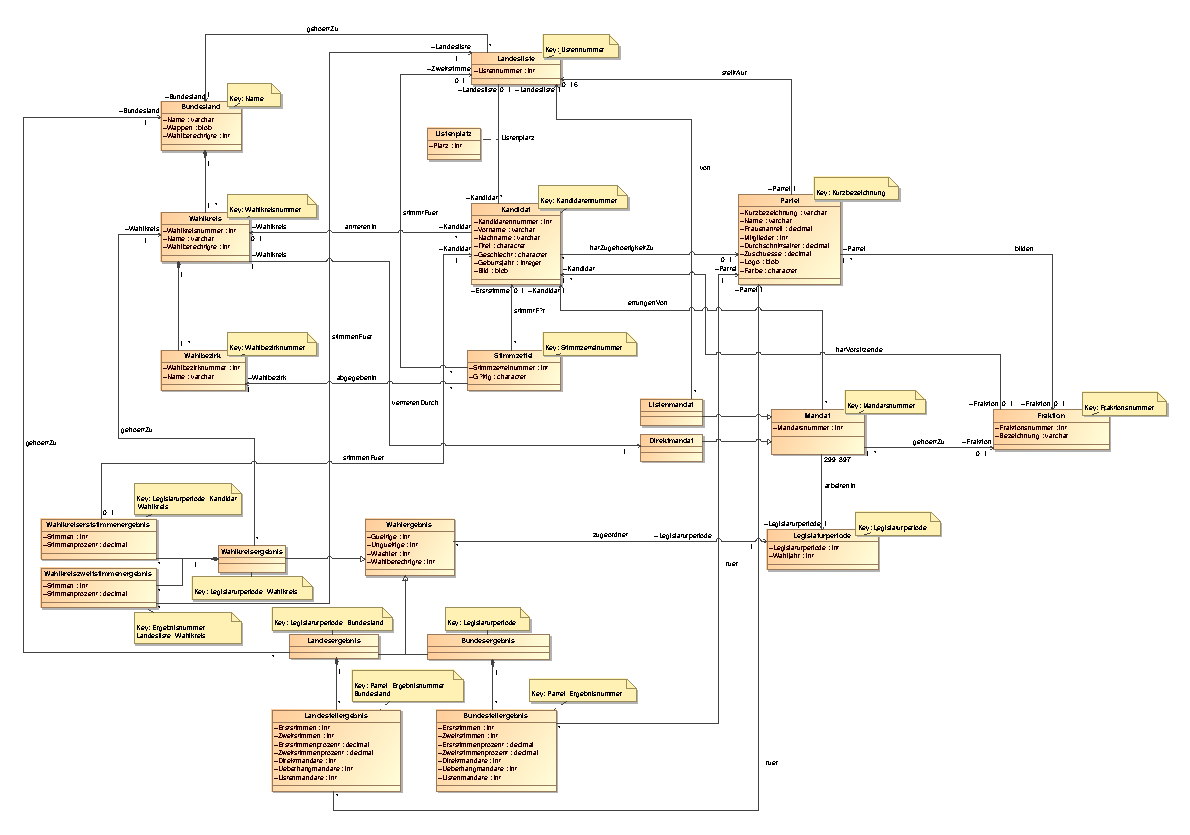
\includegraphics[scale=1,angle=90]{datenmodell.eps}

\section{Relationale Modellierung}

Im Folgenden werden die Schemata des Datenmodells dargestellt. Eine Verfeinerung wurde an geeigneten Stellen durchgeführt. Dadurch ist nicht jede Assoziation durch ein eigenes Schema vertreten.

\subsection{Schemata aus Klassen}

\begin{description}

\item[Bundesland:] \{[ \underline{Name: varchar}, Wappen: blob, Wahlberechtigte: int  ]\}

\item[Wahlkreis:] \{[ \underline{Wahlkreisnummer: integer}, Name : varchar, Bundesland: \\varchar,   ]\}

\item[Wahlbezirk:] \{[ \underline{Wahlbezirknummer: integer}, Name : varchar, Wahlkreis:\\integer  ]\}

\item[Kandidat:] \{[ \underline{Kandidatennummer: integer}, Vorname : varchar, Nachname: varchar, Titel: character, Geschlecht: character, Geburtsjahr: integer, Bild: blob, Partei: varchar  ]\}

\item[Partei:] \{[ \underline{Kurzbezeichnung: varchar}, Name : varchar, Frauenanteil: decimal, Mitglieder: integer, Durchschnittsalter: decimal, Zuschüsse: decimal, Logo: blob, Farbe: character  ]\}

\item[Landesliste:] \{[ \underline{Listennummer: integer}, Bundesland: varchar, Partei: \\varchar ]\}

\item[Fraktion:] \{[ \underline{Fraktionsnummer: integer}, Bezeichnung: varchar ]\}

\item[Legislaturperiode:] \{[ \underline{Legislaturperiode: integer}, Wahljahr: integer ]\}

\item[Listenmandat:] \{[ \underline{Mandatsnummer: integer}, Landesliste: \\integer ]\}

\item[Direktmandat:] \{[ \underline{Mandatsnummer: integer}, Wahlkreis: \\integer ]\}

\item[Mandat:] \{[ \underline{Mandatsnummer: integer}, Kandidat: integer, Legislaturperiode: integer, Fraktion: integer]\}

\item[Stimmzettel:] \{[ \underline{Stimmzettelnummer: integer}, Erststimme: integer, Zweitstimme: integer, Wahlbezirk: integer ]\}

\item[Wahlkreisergebnis:] \{[ \underline{Legislaturperiode: integer, Wahlkreis: integer}, Gültigeerststimmen: integer, Gültigezweitstimmen: integer, Wähler : integer, Wahlberechtigte: integer ]\}

\item[Wahlkreiserststimmenergebnis:] \{[ \underline{Erststimmenergebnisnummer: integer}, Legislaturperiode: integer, Kandidat: integer, Partei: varchar, Wahlkreis: integer, Stimmen: integer, Stimmenprozent: decimal ]\}

\item[Wahlkreiszweitstimmenergebnis:] \{[ \underline{Legislaturperiode: integer, Partei: varchar} \underline{, Wahlkreis: integer}, Stimmen: integer, Stimmenprozent: decimal ]\}

\item[Landesergebnis:] \{[ \underline{Legislaturperiode: integer, Bundesland: varchar}, Gültigeerststimmen: integer, Gültigezweitstimmen: integer, Wähler : integer, Wahlberechtigte: integer ]\}

\item[Landesteilergebnis:] \{[ \underline{Legislaturperiode: integer, Bundesland: varchar, Partei: varchar}, Erststimmen: integer, Erststimmenprozent: decimal, Zweitstimmen : integer, Zweitstimmenprozent: decimal, Direktmandate: integer, Überhangmandate: integer, Listenmandate: integer ]\}

\item[Bundesergebnis:] \{[ \underline{Legislaturperiode: integer}, Gültigeerststimmen: integer, Gültigezweitstimmen: integer, Wähler : integer, Wahlberechtigte: integer ]\}

\item[Bundesteilergebnis:] \{[ \underline{Legislaturperiode: integer, Partei: varchar}, Erststimmen: integer, Erststimmenprozent: decimal, Zweitstimmen : integer, Zweitstimmenprozent: decimal, Direktmandate: integer, Überhangmandate: integer, Listenmandate: integer ]\}

\end{description}

\subsection{Schemata aus Assoziationen}

\begin{description}

\item[Direktkandidatur:] \{[ \underline{Kandidat: integer}, Wahlkreis: integer ]\}

\item[Listenplatz:] \{[ \underline{Landesliste: integer, Platz: integer}, Kandidat: integer ]\}

\item[Fraktionspartei:] \{[ \underline{Partei: varchar}, Fraktion: integer ]\}

\item[Fraktionsvorsitz:] \{[ \underline{Kandidat: integer}, Fraktion: integer ]\}

\end{description}

\section{Mockups von Anwendungsfällen}

In Appendix \ref{mockups} sind exemplarisch Mockups des späteren Wahlinformationssystems gezeigt. Es wird vornehmlich Wert auf eine übersichtliche Aufbereitung bei gleichzeitig mächtiger Analysefähigkeit gelegt.

\section{Berechnung der Sitzverteilung}

\subsection{Schritt 1: Direktmandate ermitteln}

In einem ersten Schritt werden die 299 Gewinner und damit Direktmandatsträger der Wahlkreise ermittelt. Gewinner ist der Direktkandidat eines Wahlkreises der die meisten Erststimmen für sich verbuchen kann. Bei Stimmgleichheit entscheidet das Los. Unser Wahlinformationssystem ist in solchen Fällen auf eine Entscheidung des Bundeswahlleiters angewiesen.

\subsection{Schritt 2: Listenmandate ermitteln}

Die Listenmandate werden anhand des Verfahrens nach Sainte-Laguë (auch: Webster-Verfahren) berechnet. Aus designtechnischen Gründen wird das Höchst-zahlverfahren genutzt um zunächst eine bundesweite Sitzanzahl für die Parteien zu ermitteln, welche mehr als 5\% der Gesamtstimmen oder mindestens 3 Direktmandatsträger aufweisen können. Eine Hilfstabelle \texttt{UNEVEN} enthält hierfür die ersten 598 ungeraden Zahlen, welche als Divisoren für die Stimmanzahlen dienen. Mehr als 598 Divisionen sind nicht nötig, da nur 598 Listenmandate vergeben werden und in einem worst-case Szenario derselben Partei zufallen. Listing 1 zeigt den SQL-Query welcher zur Sitzbestimmung auf Bundesebene verwendet wird.

\lstset{
language=SQL,
basicstyle=\footnotesize,       % the size of the fonts that are used for the code
numbers=left,                   % where to put the line-numbers
numberstyle=\footnotesize,      % the size of the fonts that are used for the line-numbers
stepnumber=2,                   % the step between two line-numbers. If it's 1 each line will be numbered
numbersep=5pt,                  % how far the line-numbers are from the code
showspaces=false,               % show spaces adding particular underscores
showstringspaces=false,         % underline spaces within strings
frame=single,	                % adds a frame around the code
tabsize=2,	                % sets default tabsize to 2 spaces
captionpos=b,                   % sets the caption-position to bottom
breaklines=true                % sets automatic line breaking
}
\begin{lstlisting}[caption=Bestimmung der Mandate für die 17. Legislaturperiode]
WITH DIRECTMANDATES (PARTEI, MANDATES) AS (
	SELECT PARTEI, COUNT(KANDIDAT)
	FROM (DIREKTMANDAT JOIN MANDAT ON MANDAT.MANDATSNUMMER = DIREKTMANDAT.MANDATSNUMMER) JOIN KANDIDAT ON KANDIDAT.KANDIDATENNUMMER = MANDAT.KANDIDAT
	WHERE LEGISLATURPERIODE = 17
	GROUP BY PARTEI),
QUALIFYING (PARTEI, ZWEITSTIMMEN) AS (
	SELECT BUNDESTEILERGEBNIS.PARTEI, ZWEITSTIMMEN    
	FROM BUNDESTEILERGEBNIS LEFT OUTER JOIN DIRECTMANDATES ON BUNDESTEILERGEBNIS.PARTEI = DIRECTMANDATES.PARTEI
	WHERE LEGISLATURPERIODE = 17
	AND (ZWEITSTIMMENPROZENT >= 5
	OR DIRECTMANDATES.MANDATES >= 3)),
QUOTIENTS AS (
	SELECT PARTEI, CAST(ZWEITSTIMMEN AS FLOAT)/CAST(NUMBER AS FLOAT) AS QUOTIENT
	FROM QUALIFYING, UNEVEN
	ORDER BY QUOTIENT DESC
	FETCH FIRST 598  ROWS ONLY)
SELECT PARTEI, COUNT(PARTEI) AS LISTENMANDATE
FROM QUOTIENTS
GROUP BY PARTEI;
\end{lstlisting}

Nachdem eine Sitzverteilung auf Bundesebene bestimmt ist wird das selbe Verfahren verwendet um die Sitze einer Partei abhängig von den Stimmen aus den Bundesländern mit Kandidaten aus den Landeslisten zu besetzen. Dies ist in Listing 2 gezeigt. Hierbei ist zu beachten das von der errechneten Anzahl der auf Landesebene zu vergebenen Sitze erst noch die Direktmandate der Partei in diesem Bundesland abgezogen werden. Ist die Anzahl der durch Landeslisten zu vergebenden Mandate negativ, so wird dieser Überhang als Überhangmandate bezeichnet und keine Listenmandate werden vergeben, ist die Anzahl positiv werden Listenmandate nach Priorität von der Landesliste der jeweiligen Partei vergeben.

\begin{lstlisting}[caption=Bestimmung der Landesmandate für die 17. Legislaturperiode und die Partei SPD]
WITH QUOTIENTS AS (
	SELECT PARTEI, BUNDESLAND, CAST(ZWEITSTIMMEN AS FLOAT)/CAST(NUMBER AS FLOAT) AS QUOTIENT
	FROM LANDESTEILERGEBNIS, UNEVEN
	WHERE PARTEI = 'SPD'
	AND LEGISLATURPERIODE = 17
	ORDER BY QUOTIENT DESC
	FETCH FIRST 146 ROWS ONLY)
SELECT PARTEI, BUNDESLAND, COUNT(BUNDESLAND) AS LISTENMANDATE
FROM QUOTIENTS
GROUP BY BUNDESLAND, PARTEI;
\end{lstlisting}

\textbf{Hinweis:} Die vorgestellten Verfahren können unter Umständen bei Stimmgleichheit von Parteien dazu führen, dass Sitze falsch zugeordnet werden. In solchen Fällen wäre eine Losentscheidung des Bundeswahlleiters von nöten.  Wir werten diesen Fall als sehr unrealistisch und werden ihn in der Applikationslogik beachten.

\addappheadtotoc
\appendix
\newpage

\section{Mockups}
\label{mockups}

\begin{figure}[h!]
\centering
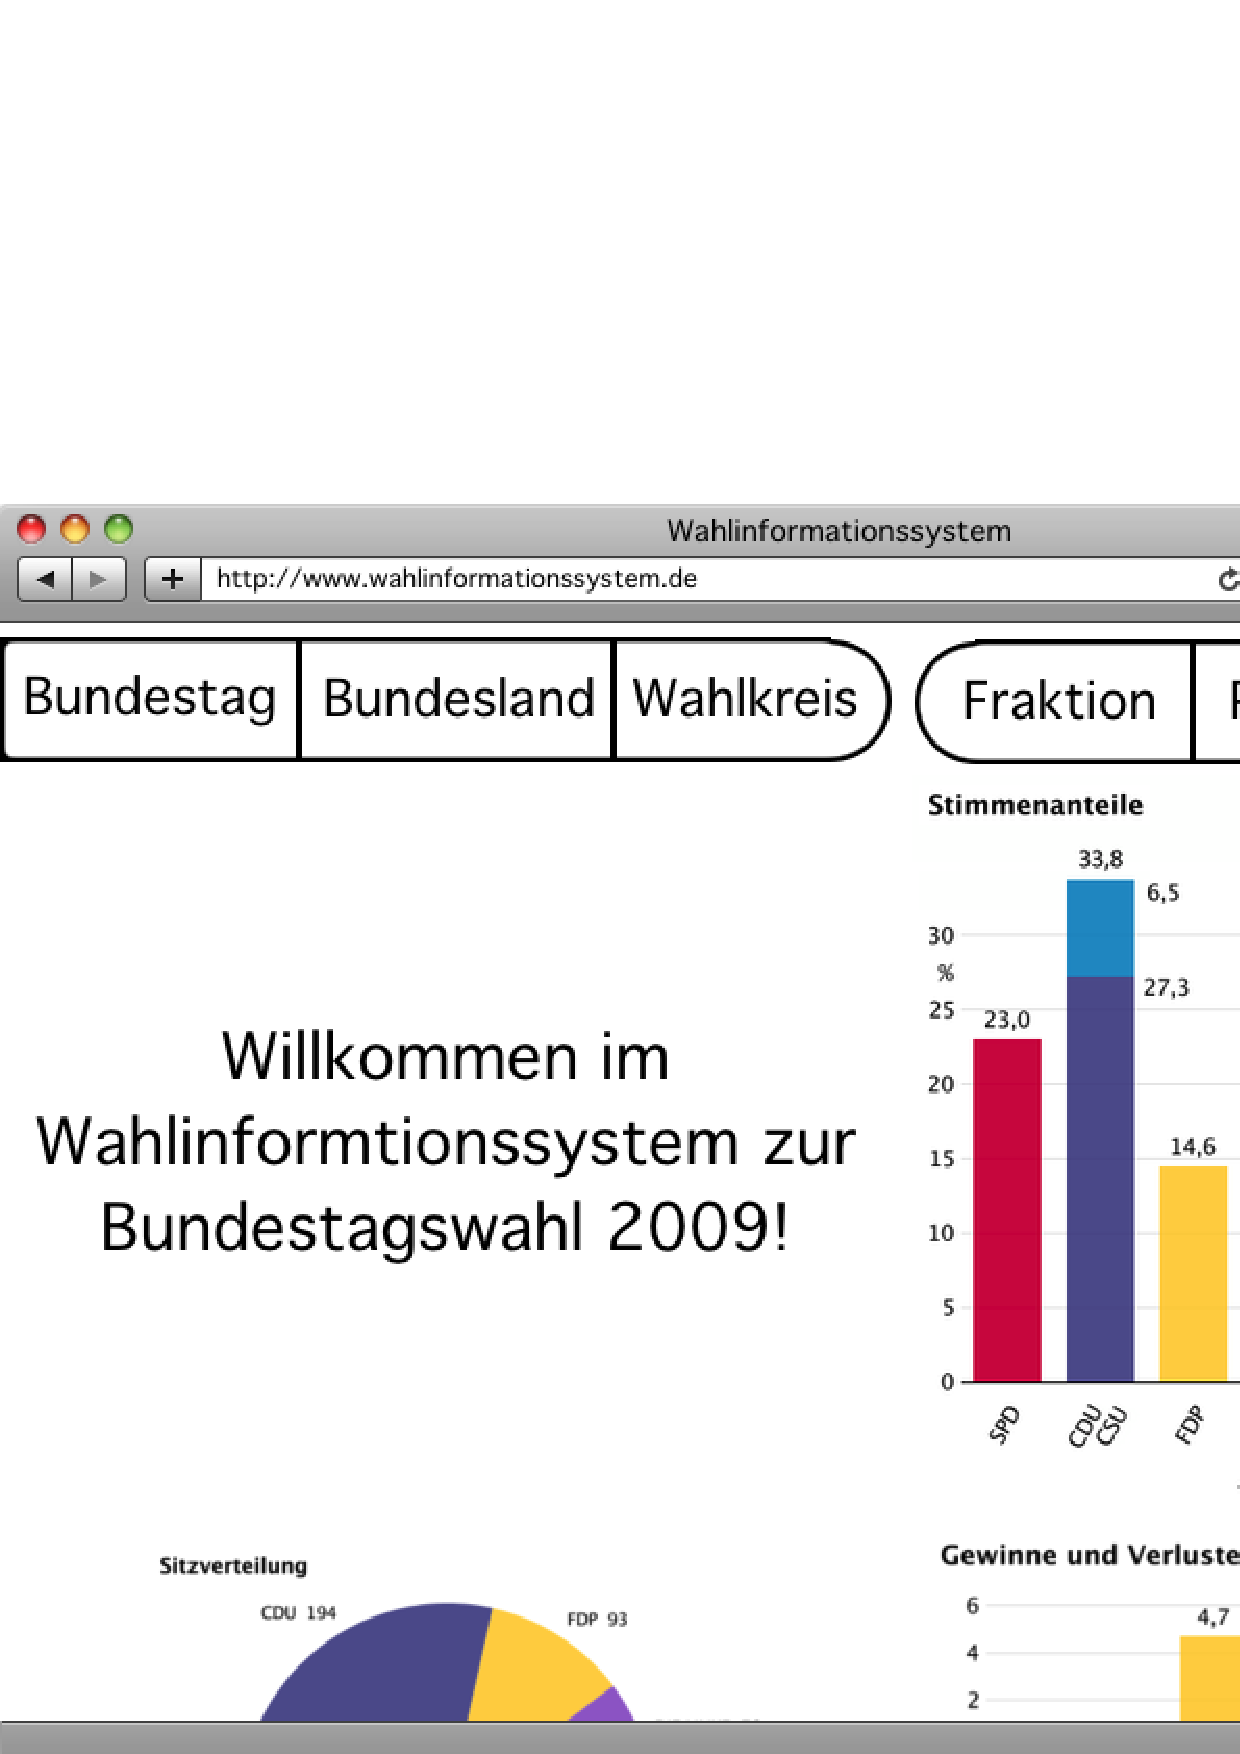
\includegraphics[scale=0.4]{Mockups/startseite}
\caption{Mockup der Startseite des Wahlinformationssystems}
\end{figure}

\begin{figure}[h!]
\centering
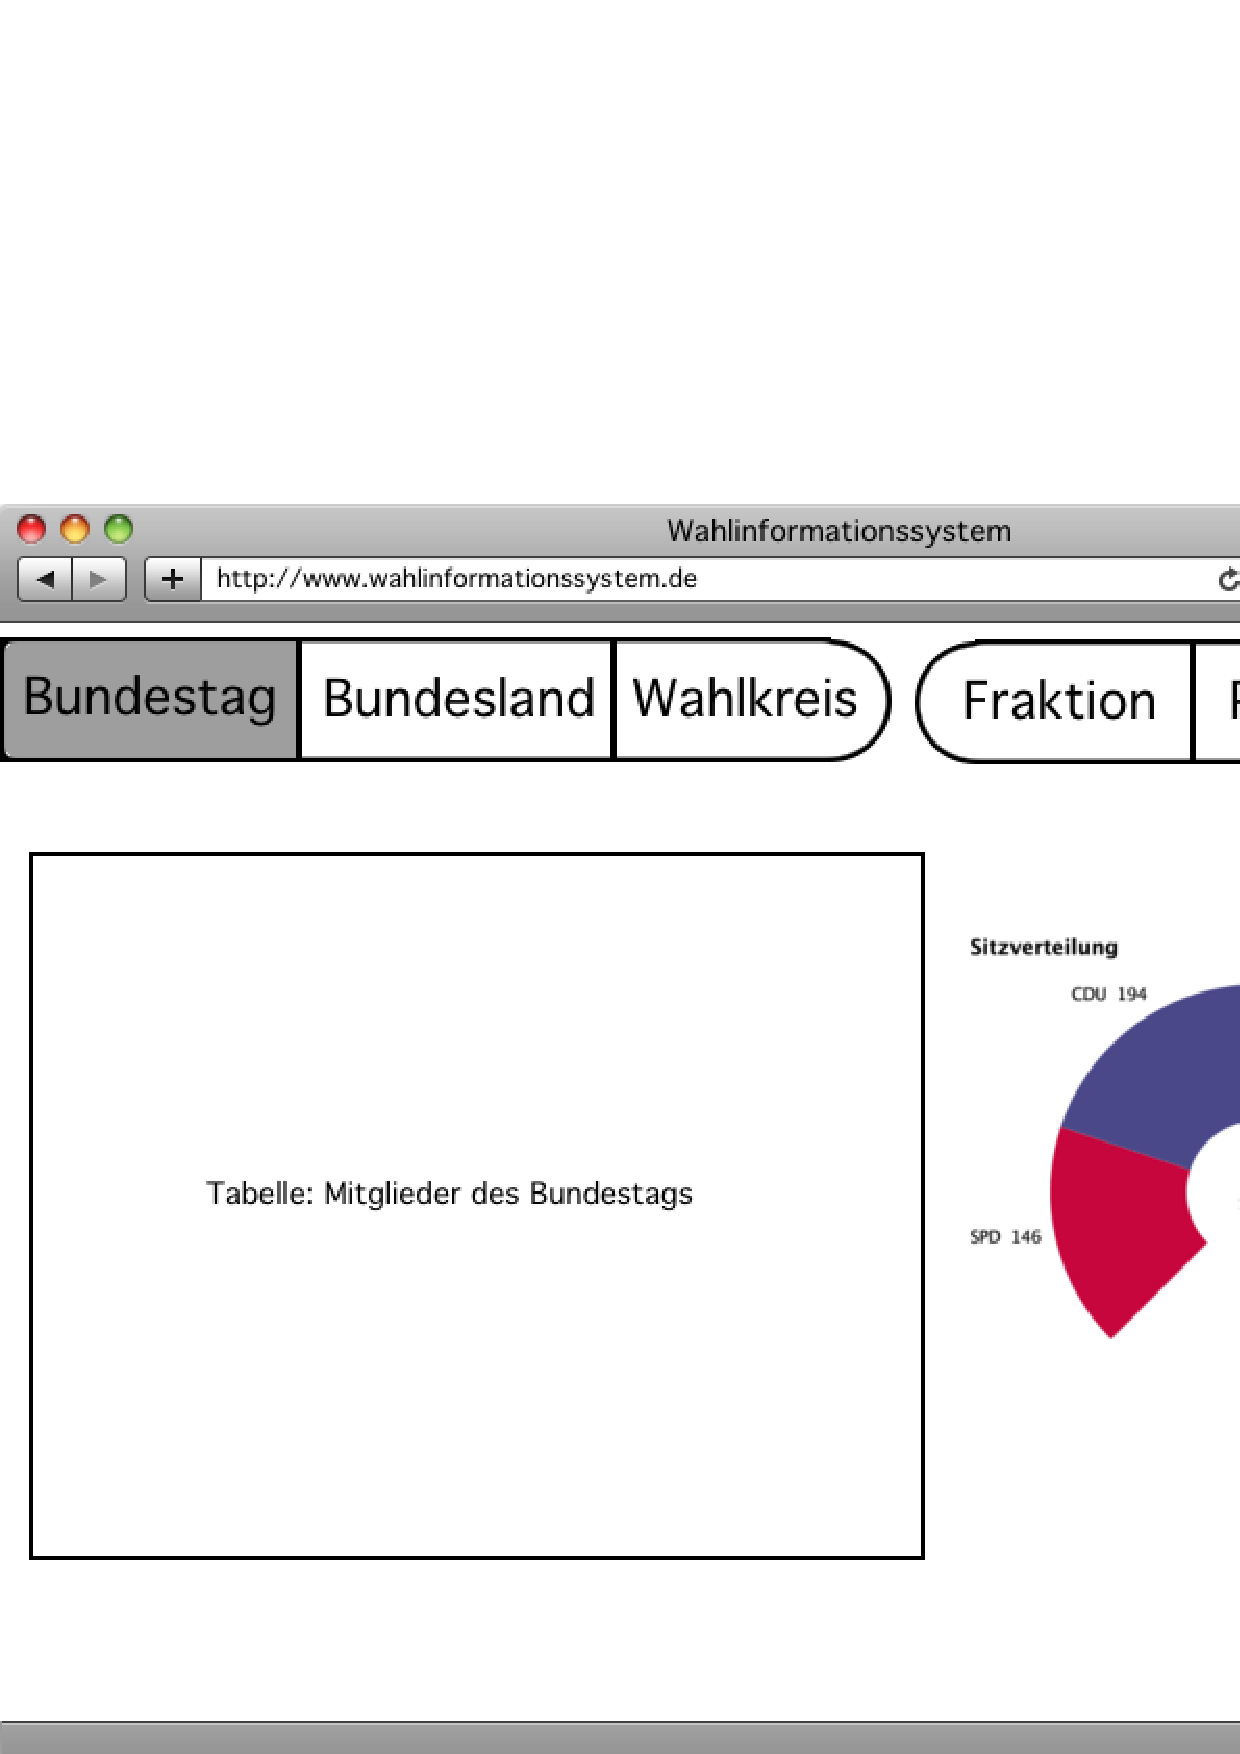
\includegraphics[scale=0.4]{Mockups/bundestag}
\caption{Ansicht des Bundestags}
\end{figure}

\begin{figure}[h!]
\centering
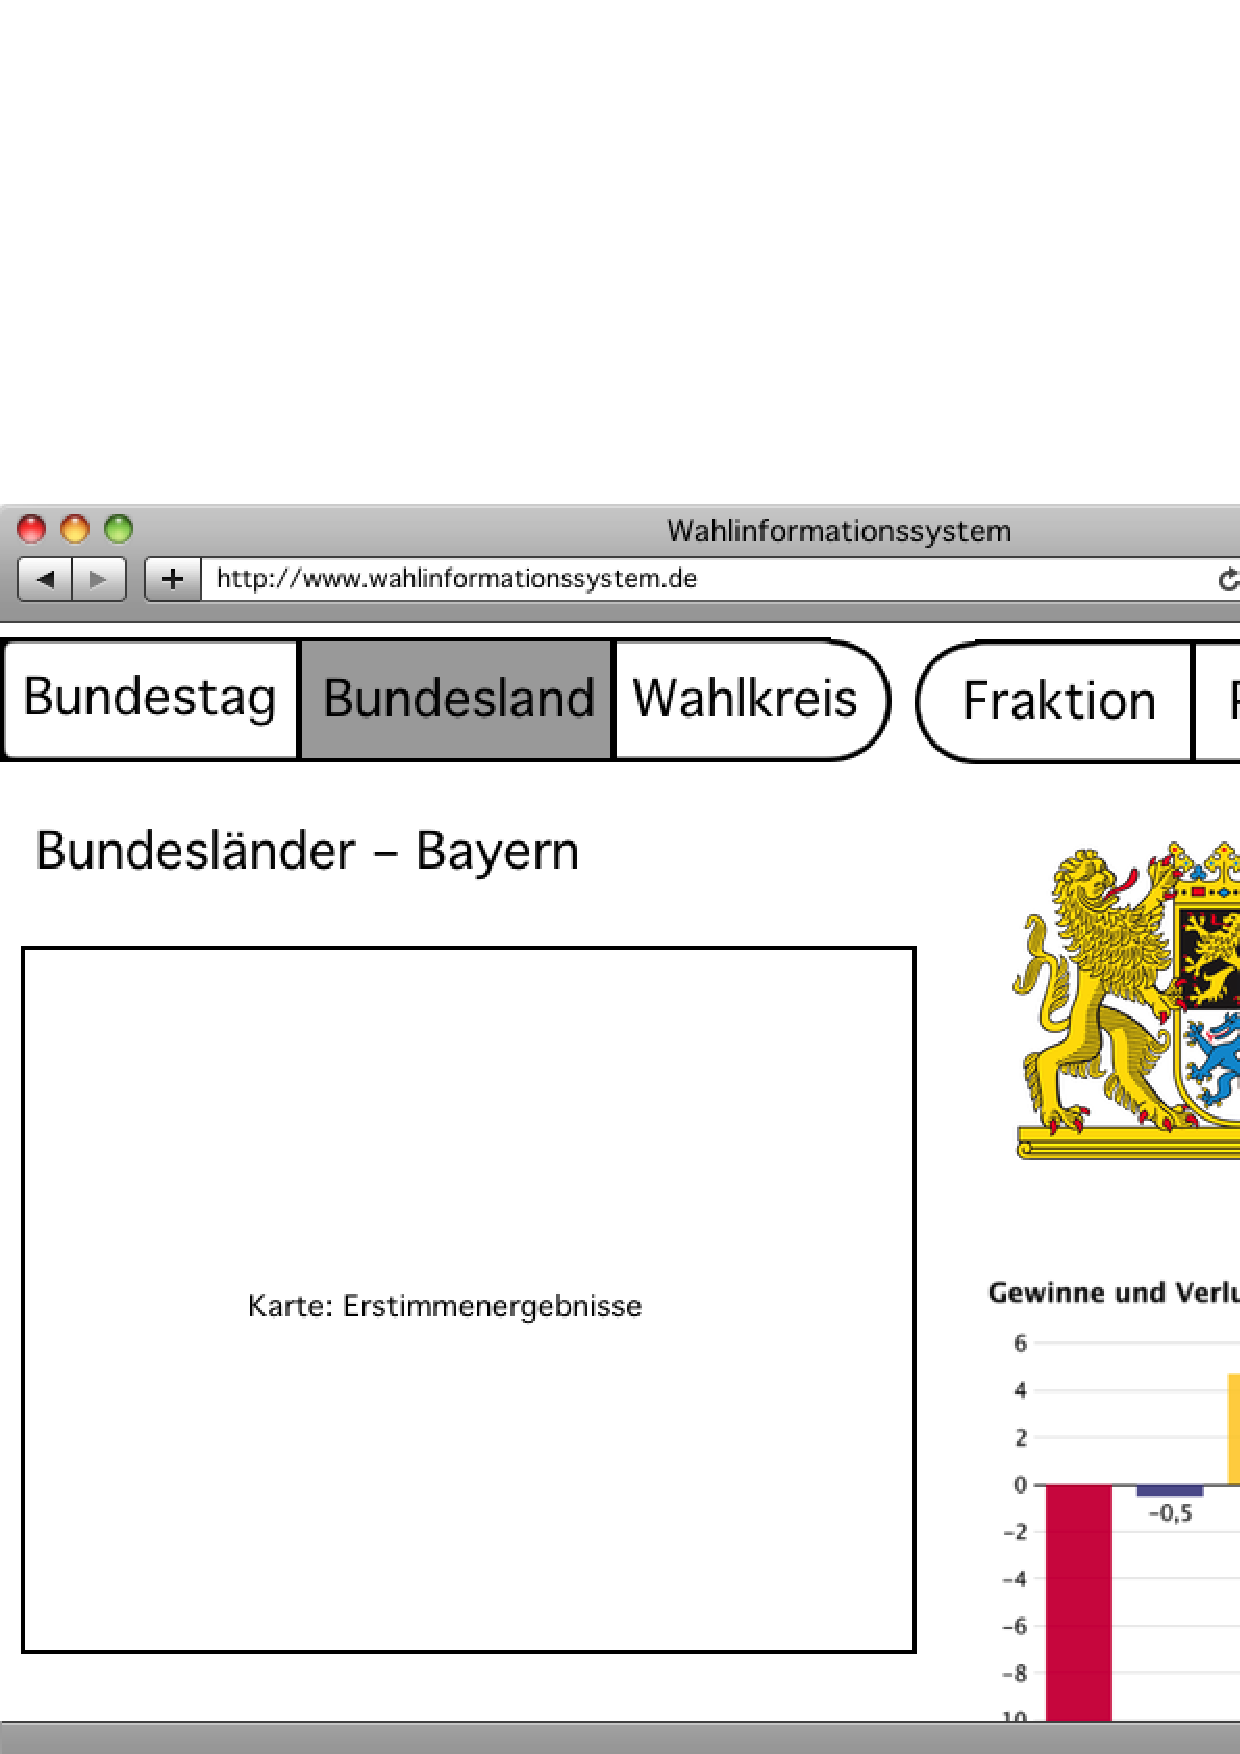
\includegraphics[scale=0.4]{Mockups/bundesland}
\caption{Ergebnisse auf Bundeslandebene}
\end{figure}

\begin{figure}[h!]
\centering
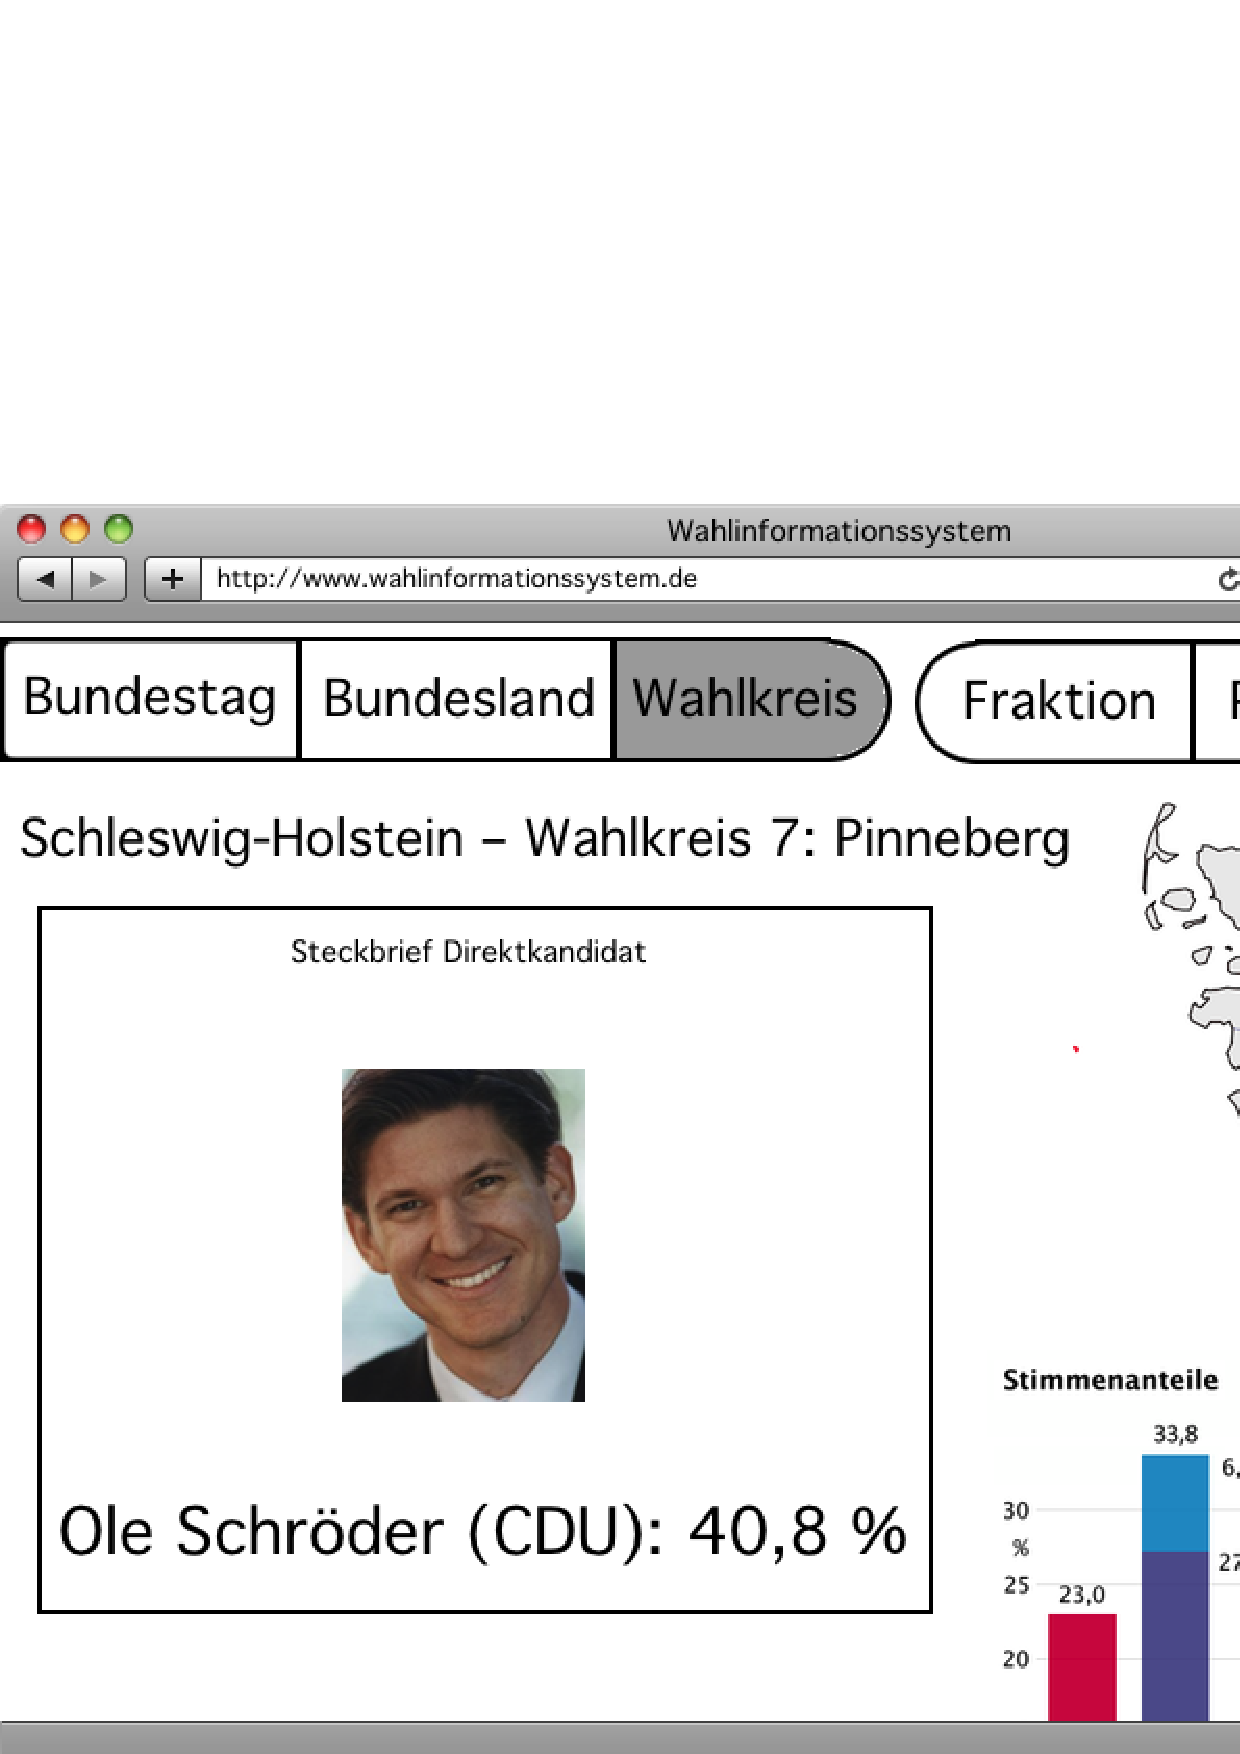
\includegraphics[scale=0.4]{Mockups/wahlkreis}
\caption{Ergebnisse auf Wahlkreisebene}
\end{figure}

\begin{figure}[h!]
\centering
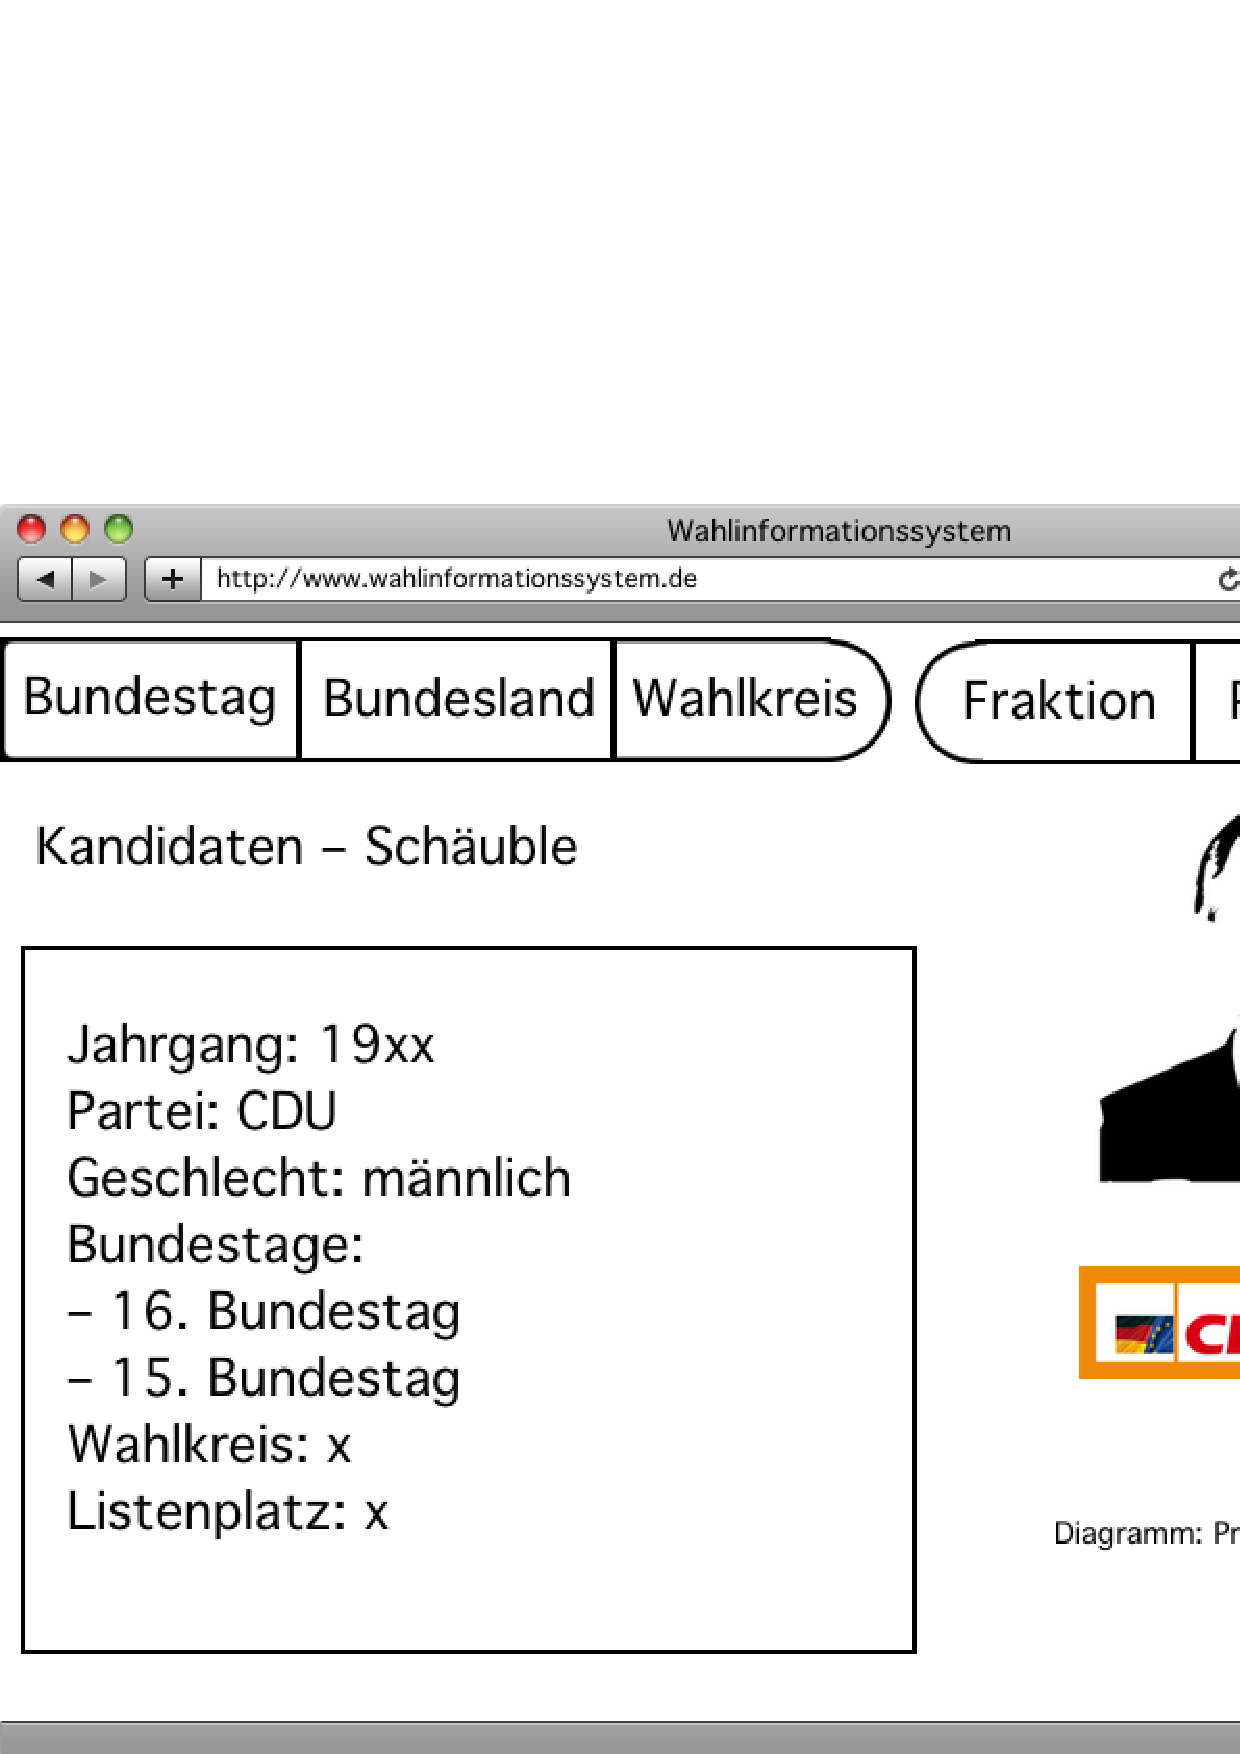
\includegraphics[scale=0.4]{Mockups/kandidat}
\caption{Detailinformationen zu den Kandidaten}
\end{figure}

\begin{figure}[h!]
\centering
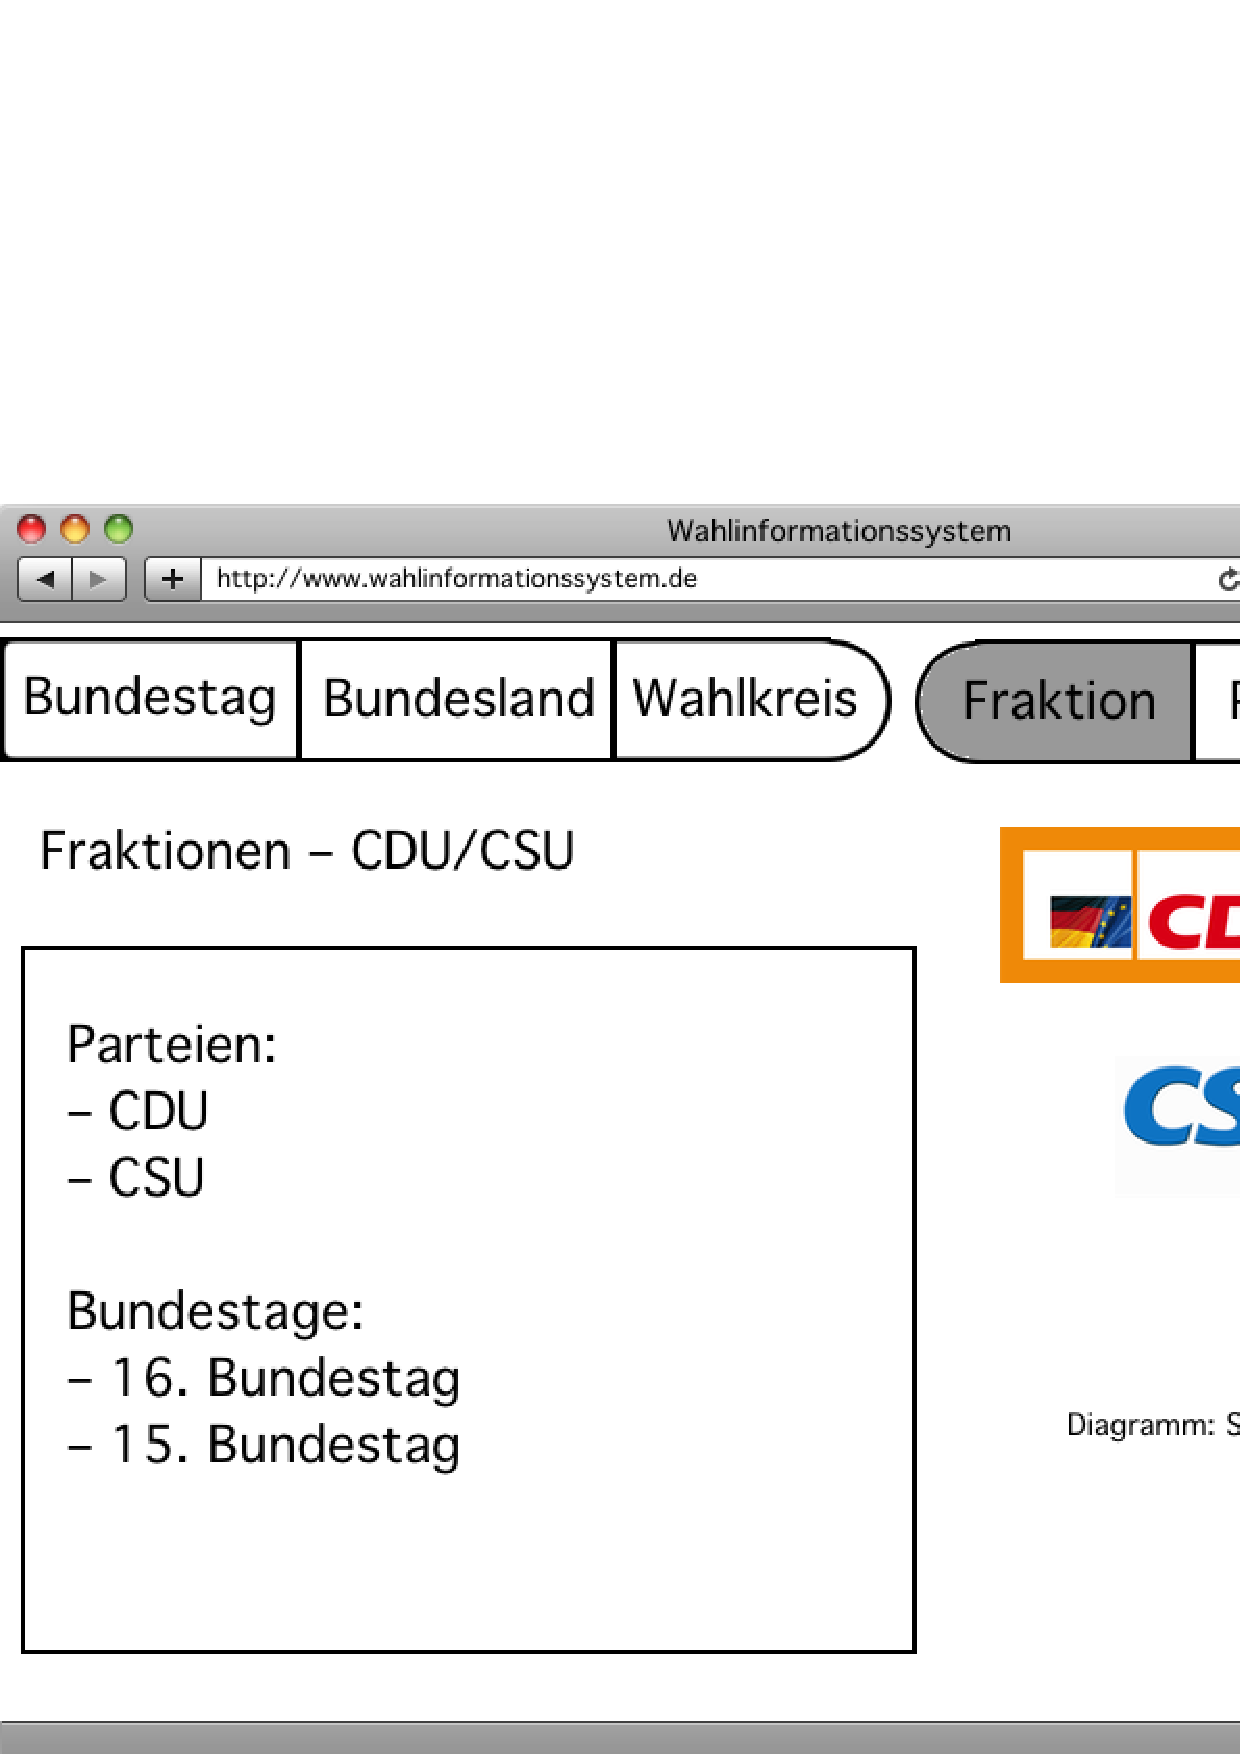
\includegraphics[scale=0.4]{Mockups/fraktion}
\caption{Detailinformationen zu den Fraktionen}
\end{figure}

\begin{figure}[h!]
\centering
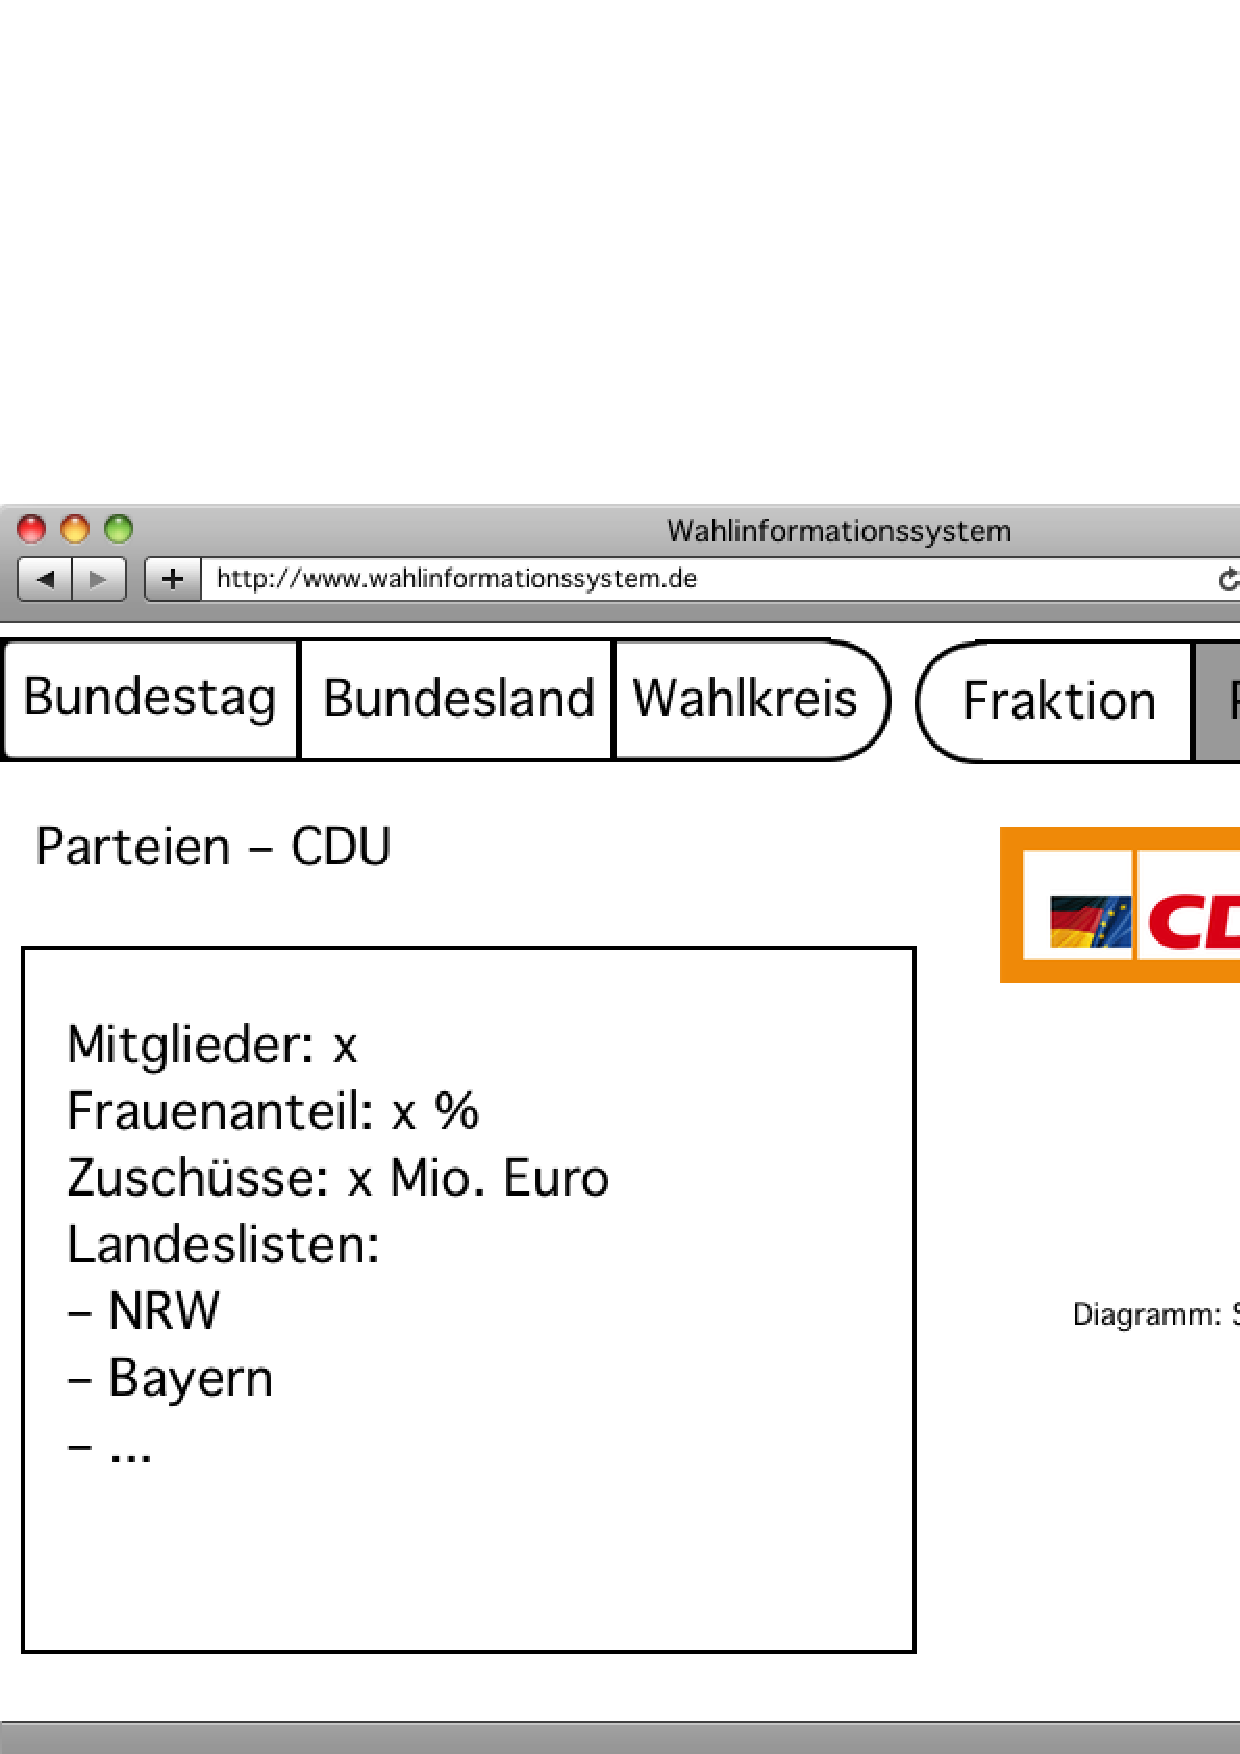
\includegraphics[scale=0.4]{Mockups/partei}
\caption{Detailinformationen zu den Parteien}
\end{figure}
\end{document}

